\ifdefined\maindoc
% Under the thesis build, main.tex owns the full \graphicspath list (it already includes
% Chapters/Introduction/figures/). \graphicspath REPLACES rather than appends, so this branch
% deliberately does nothing.
\else
\documentclass[12pt]{report}
\usepackage[a4paper,margin=1in]{geometry}
\usepackage[utf8]{inputenc}
\usepackage[T1]{fontenc}
\usepackage[british]{babel}
\usepackage{amsmath,amssymb}
\usepackage{booktabs}
\usepackage{setspace}
\usepackage{graphicx}
\usepackage{enumitem}
\usepackage{placeins}
\usepackage{hyperref}
\usepackage{array}
\usepackage[backend=biber,style=ieee,citestyle=numeric-comp,sorting=none]{biblatex}
\addbibresource{../../references.bib}
\setcounter{biburllcpenalty}{7000}
\setcounter{biburlucpenalty}{8000}
\setcounter{biburlnumpenalty}{9000}
\onehalfspacing
\graphicspath{{figures/}}
% Standalone-only fallbacks so Chapter~\ref{...} renders as the right number outside the
% main thesis. Numbers follow the agreed order after the Input Module chapter was folded into
% the Network Model chapter: 1 this chapter, 2 Background, 3 Network Model (incl. input
% processing), 4 Network Decomposition, 5 Probability, 6 Capacity Flow, 7 Critical Path,
% 8 Julia package, 9 Interface, 10 Integrated Case Study, 11 Conclusions.
\makeatletter
\newlabel{ch:lit-review}{{2}{1}{}{Doc-Start}{}}
\newlabel{ch:system-model}{{3}{1}{}{Doc-Start}{}}
\newlabel{ch:diamond-module}{{4}{1}{}{Doc-Start}{}}
\newlabel{ch:probability-toolkit}{{5}{1}{}{Doc-Start}{}}
\newlabel{ch:capacity-toolkit}{{6}{1}{}{Doc-Start}{}}
\newlabel{ch:critical-path}{{7}{1}{}{Doc-Start}{}}
\newlabel{ch:julia-package}{{8}{1}{}{Doc-Start}{}}
\newlabel{ch:front-end}{{9}{1}{}{Doc-Start}{}}
\newlabel{ch:integrated-case-study}{{10}{1}{}{Doc-Start}{}}
\newlabel{ch:conclusions}{{11}{1}{}{Doc-Start}{}}
\makeatother
% The integrated case study network is not yet chosen. \CaseStudyNetwork is deliberately left
% undefined in main.tex so that the build fails until it is. For a standalone compile of this
% chapter only, a visible placeholder is defined here.
\newcommand{\CaseStudyNetwork}{[CASE STUDY NETWORK]}
\begin{document}
\title{Introduction}
\fi

\section{Motivation}
\label{sec:intro-motivation}

Many civil infrastructure systems are process systems. They take a resource in at one end,
transform or transport it through a sequence of connected stages, and deliver it at the
other. A water treatment works, for instance, abstracts raw water from a river or a borehole,
passes it through screening, coagulation, filtration and disinfection, and pumps the treated
water into a distribution network that carries it to consumers. Each stage depends on the
stages upstream of it, and the output of the works depends on all of them. Systems of this
kind, in which a resource moves through a sequence of stages towards a delivery goal, are
referred to in this thesis as goal-oriented process systems. Where the direction of flow
through such a system is fixed and there is no feedback in normal operation, the system can be
modelled as a directed acyclic graph (DAG), with components as nodes and dependencies as
directed edges.

Given such a model, several different questions can be asked of it, and three are addressed in
this thesis. The first is a question of reliability: with what probability does supply reach a
given point when components can fail? The second is a question of capacity: how much can the
system deliver, and which components limit it? The third is a question of schedule: when does
a dependent sequence of operations complete, and which operations can be delayed without
delaying the whole? Each question has a method of its own. Network reliability analysis
answers the first \cite{billinton1992network}, the maximum-flow and minimum-cut theory of the
1950s answers the second \cite{ford1956}, and the critical path method of the same decade
answers the third \cite{kelley1959critical}. The three methods have separate literatures and
separate software, and each is normally applied to its own model of the system. However, the
topology is the same in all three. What changes with the analysis goal is the meaning of the
value attached to a component: a failure probability, a throughput limit or a duration. In the
framework developed here the three analyses are therefore independent readings of one network
model, each with its own inputs and its own algorithm, and the model is entered once.

The values attached to the components are rarely known precisely. Aleatory uncertainty is the inherent variability of a quantity, such as
the time to failure of a pump across a population of identical pumps, and is well described by a
probability distribution. Epistemic uncertainty is a lack of knowledge about the quantity, and
can in principle be reduced by collecting more data. For example, a failure probability estimated from three recorded failures, a capacity quoted
as a nameplate rating with a tolerance, or a duration elicited from an engineer who will commit
to a range but not to a number are all cases of the second kind. Describing epistemic uncertainty with a single value, or with a precise
probability distribution, requires assumptions that the data do not support. Generalised
probabilistic methods have been developed to avoid this. An interval bounds an unknown quantity
between two values without assuming anything about where it lies between them. A probability
box, or p-box, bounds an unknown distribution between a lower and an upper cumulative
distribution function, and so carries partial statistical knowledge without fixing a
distribution \cite{ferson2003constructing,williamson1990probabilistic}. However, all three methods named above consume a single value for each input. In practice an
analyst therefore chooses a point value and treats the remaining uncertainty in a separate
sensitivity study, if at all.
This thesis instead propagates intervals and p-boxes through the network computation
itself, so that the result carries the same kind of bound as the inputs. For the reliability
question in particular this has rarely been done, because exact network reliability
is \#P-hard \cite{valiant1979complexity,ball1986computational} and every exact method in
common use, from reliability block diagrams to binary decision diagrams, is built on
point-valued component probabilities.

This thesis develops the Information Propagation Framework (IPF). The framework provides one
DAG model of a system on which reliability, capacity and schedule analysis are computed,
propagates interval and p-box inputs through each analysis as far as the mathematics of that
analysis allows, and is provided as a Julia package together with a no-code user interface for
non-technical users. Figure~\ref{fig:intro-framework-overview} shows the framework as a set of
layers. The network model, the input processing that builds it and the decomposition module
that identifies its reconvergent structure are built once per system. The three analysis
toolkits read the same graph object. The probability toolkit propagates deterministic values,
intervals and p-boxes; the critical path toolkit propagates deterministic values and
intervals; the capacity toolkit is point-valued in the present work. The package and the
interface are the delivery layer. The three toolkits are the analyses developed in this thesis. A further analysis would read
the same graph object.

\begin{figure}[htbp]
  \centering
  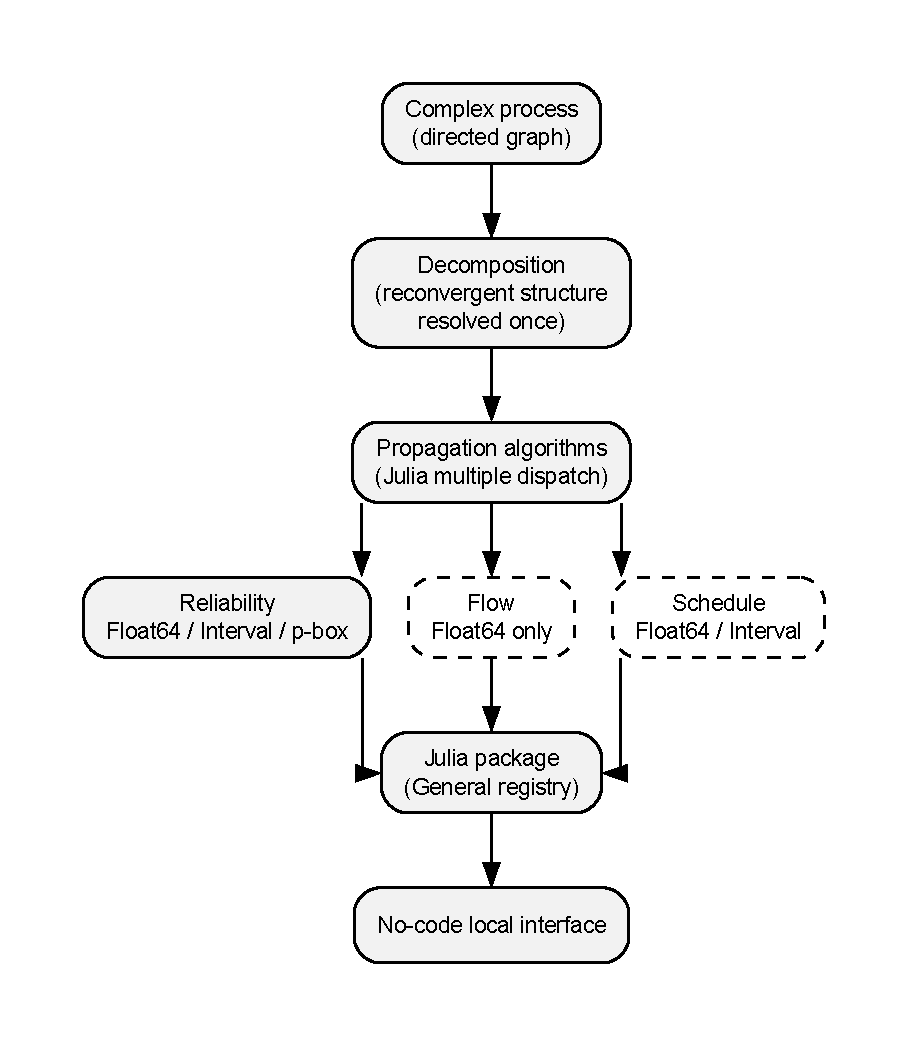
\includegraphics[width=0.6\textwidth]{fig01_framework_overview/fig01_framework_overview.pdf}
  \caption{The framework as a set of layers. The network model and its decomposition are built
    once per system. The three analysis toolkits read the same graph object, and each carries
    the uncertainty support shown: deterministic values, intervals and probability boxes in the
    probability toolkit; deterministic values and intervals in the critical path toolkit;
    deterministic values only in the capacity toolkit. The package and the interface deliver the
    framework.}
  \label{fig:intro-framework-overview}
\end{figure}

\section{Problem Statement and Research Questions}
\label{sec:intro-problem}

Several engineering software tools run more than one kind of analysis against one shared
network object. \texttt{pandapower}, for instance, runs power flow, optimal power flow,
state estimation, topological search and short-circuit calculation against one graph of buses
and lines \cite{thurner2018pandapower}. However, no tool or method found in the review of
Chapter~\ref{ch:lit-review} combines source-to-node reliability, capacitated flow and activity
scheduling on one network representation. The closest work pairs two of the three. Huang, Huang
and Lin compute the exact probability that a project completes within a time and a budget
constraint, which pairs reliability with schedule, from discrete point-valued activity states
\cite{huang2020exact}. Tong's dissertation investigates infrastructure flow networks in terms
of both connectivity and flow capacity, which pairs reliability with flow, using a point-valued
propagation method throughout \cite{tong2021infrastructure}. Furthermore, in neither case, and in none of the commercial or open-source tools reviewed, is
an interval or a p-box propagated natively through the computation, and none of them is
delivered in a form that a user can operate without writing code.

Following these considerations, the research questions addressed in this thesis are the
following:

\begin{enumerate}
  \item Can one DAG model of a complex process serve reliability, capacity and schedule
    analysis of the same system, so that the topology is entered once and read three times?
  \item The redundancy that makes a system robust is also what makes its exact analysis
    expensive, because routes that diverge and reconverge share components. Can this structure
    be identified once, independently of any particular analysis, and reused?
  \item Can exact source-to-node reliability be computed when component probabilities are
    given as intervals or as p-boxes, what is guaranteed of the result in each case, and what
    does the computation cost relative to the established exact methods?
  \item Which of the quantities of critical path analysis remain exactly computable when
    durations are intervals, and at what cost, given that the general problem is NP-hard
    \cite{chanas2002complexity}?
  \item Can these analyses be provided to an engineer who does not program, without the system
    model leaving the engineer's machine?
\end{enumerate}

\section{Objectives}
\label{sec:intro-objectives}

The aim of this work is a framework for the analysis of complex processes modelled as DAGs, in
which the treatment of uncertain inputs is chosen by the state of knowledge about the system.
The limits of the tool should not force that choice. The objectives are:

\begin{itemize}
  \item To define a network model general enough that reliability, capacity and schedule
    analysis are each a reading of the same object, and to build that object from the file
    formats in which infrastructure data commonly arrives.
  \item To develop exact analysis methods for each of the three readings, and to extend each to
    interval and p-box inputs as far as the mathematics of that reading allows.
  \item To validate every exact result against an independent computation, and to measure
    where each method stops being practical.
  \item To provide the framework as a documented Julia package and as a no-code user interface
    built on that package.
\end{itemize}

\section{Contributions}
\label{sec:intro-contributions}

The main contributions of this thesis are the following.

\begin{enumerate}
  \item \textbf{A network model and its graph object.} A system is modelled as a finite DAG
    with sources, sinks, forks and joins. The graph object built from it carries, in addition
    to the topology, a layered topological order, the ancestor and descendant closure of every
    node, and the node roles, all computed in one pass. Every analysis in the framework reads
    this object. An input module builds it from edge lists and adjacency matrices, and attaches
    analysis inputs from a JSON contract that declares the value form (deterministic, interval
    or p-box) and the analysis class.
  \item \textbf{A network decomposition module.} The module identifies every instance of a
    subgraph pattern in the network, with the diamond, a fork whose paths reconverge at a
    downstream join, as its default pattern. Each unique diamond is stored once, as a graph
    object of the same form as the network, and the identification is proved to be complete,
    deterministic and terminating. The probability toolkit is the consumer of this module in
    the present work.
  \item \textbf{The Probability Propagation Toolkit.} Its algorithm, the Probability
    Propagation Algorithm (PPA), computes for every node the exact probability that the node
    operates and is reached from a source, in one pass over the layered order, resolving each
    reconvergence by conditioning on the diamond identified there. The same propagation is
    applied to deterministic, interval and p-box inputs. For deterministic inputs it returns
    the exact reliability; for intervals it returns the exact range, by a monotonicity
    argument; for p-boxes it returns sound bounds on the distribution of the reliability. The
    results are validated against binary decision diagrams, exhaustive path enumeration and
    Monte Carlo simulation on a corpus of 129 random networks, structured families, benchmark
    networks from the literature and a real medical logistics network.
  \item \textbf{The Capacity Flow Toolkit.} For point-valued capacities the toolkit computes
    maximum throughput, minimum cuts, saturated edges, single points of failure, degradation
    and upgrade thresholds and path-disjoint redundancy, with every solution checked for
    feasibility, conservation and max-flow min-cut agreement.
  \item \textbf{The Critical Path Toolkit, generalised over the propagated quantity.} The
    classical critical path method is one instance of a family of analyses defined by a pair
    of operators. A backward pass exists only for pairs whose algebra supports one. For
    interval durations the forward quantities are computed exactly by two runs at the corners
    of the input box, and the floats are computed exactly by a domination split that reduces
    the enumeration from every uncertain duration to the durations that can bypass the node in
    question.
  \item \textbf{Delivery as a package and an interface.} The framework is a Julia package, and
    the package is the server behind a browser interface that runs entirely on the user's
    machine. The interface accepts the same files the package reads and returns results in the
    same value form they were given in.
\end{enumerate}

\section{Outline of the Thesis}
\label{sec:intro-structure}

Chapter~\ref{ch:lit-review} reviews the representations of uncertainty used in engineering
analysis, the exact methods for network reliability, flow and scheduling, the tools and methods
that combine more than one of these analyses on one network, and the patterns in which
engineering analysis software is delivered to its users.

In Chapter~\ref{ch:system-model} the network model is defined. Components become nodes and
dependencies become directed edges, the acyclicity assumption is discussed, and the roles of
sources, sinks, forks and joins are given their physical reading. The chapter then establishes
the layered order and the closures that every later algorithm depends on, describes how a model
is built from the heterogeneous files in which real systems are described, and states the
assumptions that all later results are conditional on.

Chapter~\ref{ch:diamond-module} presents the network decomposition module. The diamond subgraph
is defined, the identification algorithm is described, and its completeness, determinism and
termination are proved. Worked examples trace the algorithm on nested and factorised
reconvergence.

Chapter~\ref{ch:probability-toolkit} presents the Probability Propagation Toolkit. The chapter
shows why a local update fails at a reconvergent join, proves that conditioning on the diamond
repairs it, and extends the propagation to intervals and p-boxes. The method is validated
against an independent exact oracle, its cost is analysed and measured against binary decision
diagrams, and it is applied to a conceptual medical drone delivery network for Scotland
\cite{jones2025conceptual}.

Chapter~\ref{ch:capacity-toolkit} presents the Capacity Flow Toolkit, organised around the
questions it answers: throughput, binding cuts, the most damaging failures, degradation and
upgrade thresholds, redundancy and single points of failure. The chapter states the point-valued
scope of the toolkit and demonstrates it on a benchmark network under two capacity
configurations.

Chapter~\ref{ch:critical-path} presents the Critical Path Toolkit. Analysis modes are defined
by operator pairs, the forward and backward kernels are given, and the interval scheme and the
domination split are proved. The toolkit is applied to a benchmark project network from the PSPLIB library under
three readings of one set of inputs, and the exact interval floats are compared with the
conservative enclosure on the same instance.

Chapter~\ref{ch:julia-package} describes the implementation of the framework in Julia: the
types of the graph object and why a purpose-built object was preferred to the language's
general graph library, the value helpers over which the propagation is generic, the server, and
the delivery of the package through the Julia General registry.

Chapter~\ref{ch:front-end} presents the no-code interface, its local client and server
architecture, the contract between the interface and the package, and the commitment that no
data leaves the user's machine.

In Chapter~\ref{ch:integrated-case-study} the complete framework is applied to
\CaseStudyNetwork, running reliability, capacity and schedule analysis on one model through
the interface. Chapter~\ref{ch:conclusions} summarises the work and discusses the directions
in which it can be extended.

\section{Publications}
\label{sec:intro-publications}

The following papers have been published, submitted or are in preparation on the basis of the
research reported in this thesis:

\begin{itemize}
  \item Ohiani, T. and Patelli, E. (2023). ``The Information Propagation Method for Efficient
    Network Reliability Analysis.'' \textit{2023 7th International Conference on System
    Reliability and Safety (ICSRS)}, 580--584. The method published under this name is the
    Probability Propagation Algorithm of the Probability Propagation Toolkit, Chapter~\ref{ch:probability-toolkit}.
  \item Ohiani, T. and Patelli, E. Journal paper on exact and imprecise network reliability by
    probability propagation, submitted to \textit{Reliability Engineering \& System Safety}
    (under revision).
  \item Ohiani, T. and Patelli, E. Conference paper on the no-code local interface, (in preparation for ESREL 2026).
  \item Conference paper on the Julia package, (in preparation).
\end{itemize}

\ifdefined\maindoc
% do nothing
\else
\printbibliography
\end{document}
\fi